\documentclass{beamer}
%\usepackage[latin1]{inputenc}
%\usepackage{lmodern}
\usepackage{times}
\usepackage[T1]{fontenc}
\usepackage{graphicx}
\usepackage{bm}
\usepackage{tikz}
\usepackage{verbatim}
\usepackage{amsmath}
\usepackage{booktabs}
\usepackage[small,labelformat=empty]{caption}
\usepackage{url}
\usepackage{colortbl}
\usetikzlibrary{automata,positioning}

\usetheme{Frankfurt}
%\usetheme{Warsaw}
\title[Title of presentation]{Title of presentation\\
{\small possibly subtitle}
}
\author[author name]
{further information <\url{can-include.urls}>}
\institute[Fnord GmbH]{}
\date{23.5.1984 - 42.5.1984}

\begin{document}

\begin{frame}{Overview}
	\begin{tikzpicture}
		\draw[white] (-2.1,.5) rectangle (9, -7);

		% individual modules
		\node[rectangle,draw=black,minimum height=.75cm,minimum width=3cm,above right] at (0,-1) {time\_buffer};
		\node[rectangle,draw=black,minimum height=.75cm,minimum width=2.1cm,above right] at (.9,-2) {time\_date};
		\node[rectangle,draw=black,minimum height=.75cm,minimum width=2.1cm,above right] at (.9,-3) {alarm};
		\node[rectangle,draw=black,minimum height=.75cm,minimum width=2.1cm,above right] at (.9,-4) {countdown};
		\node[rectangle,draw=black,minimum height=.75cm,minimum width=3cm,above right] at (5,-3) {display\_driver};
		\node[rectangle,draw=black,minimum height=.75cm,minimum width=5cm,above right] at (0,-6) {mode\_fsm};

		% clk/reset signals (enable_gen)
		\only<2> {
			\draw[white!50!black,line width=2pt,->] (-2,-6.3) -- (6,-6.3) ->  (6,-3);
			\draw[white!50!black,line width=2pt,->] (-.5,-6.3) -- (-.5,-1) -> (0,-1);
			\draw[white!50!black,line width=2pt,->] (-.5,-2) -> (.9,-2);
			\draw[white!50!black,line width=2pt,->] (-.5,-3) -> (.9,-3);
			\draw[white!50!black,line width=2pt,->] (-.5,-4) -> (.9,-4);
			\draw[white!50!black,line width=2pt,->] (-.5,-6) -> (0,-6);
			\draw[white!50!black,line width=2pt,->] (-.5,-4.5) -- (4,-4.5) -> (4,-4);
			\node[rectangle,below right] at (-2,-6.3) {enable\_gen};
		}

		% time signals
		\only<3-> {
			\draw[red!50!black,line width=2pt,->] (-1,-.625) -- (0,-.625);
			\draw[red!50!black,line width=2pt,->] (.5,-1) -- (.5,-1.5) -> (.9,-1.5);
			\draw[red!50!black,line width=2pt,->] (.5,-1) -- (.5,-2.5) -> (.9,-2.5);
			\draw[red!50!black,line width=2pt,->] (.5,-1) -- (.5,-3.5) -> (.9,-3.5);
			\node[rectangle,above right] at (-2,-.625) {dcf77\_eval};
		}

		% key status signals
		\only<4-> {
			\draw[green!50!black,line width=2pt,->] (-1,-1.75) -- (-.25,-1.75) -- (-.25,-1.75) -> (.9,-1.75);
			\draw[green!50!black,line width=2pt,->] (-1,-1.75) -- (-.25,-1.75) -- (-.25,-2.75) -> (.9,-2.75);
			\draw[green!50!black,line width=2pt,->] (-1,-1.75) -- (-.25,-1.75) -- (-.25,-3.75) -> (.9,-3.75);
			\draw[green!50!black,line width=2pt,->] (-1,-1.75) -- (-.25,-1.75) -- (-.25,-5.625) -> (0,-5.625);
			\node[rectangle,above right] at (-2,-1.75) {key\_control};
		}

		% display data signals
		\only<5-> {
			\draw[line width=2pt,->] (3,-1.625) -> (4, -1.625);
			\draw[line width=2pt,->] (3,-2.625) -> (4, -2.625);
			\draw[line width=2pt,->] (3,-3.625) -> (4, -3.625);
			\draw[line width=2pt,->] (4.5,-2.625) -> (5, -2.625);
		}

		\only<6-> {
			% status signals modules -> fsm
			% only needed for alarm since we dropped the modified signal
			% \draw[->] (3,-1.375) -- (3.4,-1.375) -> (3.4,-5.25);
			\draw[->] (3,-2.375) -- (3.3,-2.375) -> (3.3,-5.25);
			% \draw[->] (3,-3.375) -- (3.2,-3.375) -> (3.2,-5.25);

			% control signals fsm -> modules
			\draw[->] (3.8,-5.25) -- (3.8,-1.875) -> (3,-1.875);
			\draw[->] (3.7,-5.25) -- (3.7,-2.875) -> (3,-2.875);
			\draw[->] (3.6,-5.25) -- (3.6,-3.875) -> (3,-3.875);

			% mux ctl
			\draw[->] (4.25,-5.25) -> (4.25,-3.75);
		}

		\only<7-> {
			% misc outputs from modules (alarm, timer)
			\draw[blue!70!black,line width=2pt,->] (3,-2.25) -- (3.5,-2.25) -- (3.5,-.5) -> (9,-.5);
			\draw[blue!70!black,line width=2pt,->] (3,-3.25) -- (3.5,-3.25) -- (3.5,-.5) -> (9,-.5);

			% \node[rectangle,draw=black,above right] at (5,-1.75) {sw\_on<='0'};
			% \draw[blue!70!black,line width=2pt,->] (6,-1.2) -- (6,-.5) -> (9,-.5);

			% display control lines
			\draw[blue!70!black,line width=2pt,->] (8,-2.625) -> (9,-2.625);
		}

		% mux
		\draw (4,-1.25) -- (4.5, -1.75) -- (4.5,-3.5) -- (4,-4) -- cycle;
		\node[rotate=90] at (4.25,-2.625) {display\_mux};

		% top level module
		\draw[dashed,gray] (-.75,0) rectangle (8.5, -6.25);
	\end{tikzpicture}
\end{frame}

\begin{frame}{Workload Distribution}
	\begin{columns}
		\begin{column}{5cm}
			\begin{tabular}{lll}
				\rowcolor{white!80!red}             time\_buffer      & Mathias   \\
				\rowcolor{white!80!red}             display\_driver   & Mathias   \\
				\rowcolor{yellow!50!green!20!white} mode\_fsm         & Fabian    \\
				\rowcolor{yellow!50!green!20!white} display\_mux      & Fabian    \\
				\rowcolor{white!80!yellow}          mode\_time\_date  & Tobi      \\
				\rowcolor{white!80!orange}          mode\_alarm       & Sophia    \\
				\rowcolor{white!80!yellow}          mode\_countdown   & Tobi      \\
				\rowcolor{white!80!orange}          uhrenbaustein     & Sophia
			\end{tabular}
		\end{column}
		\begin{column}{6cm}
			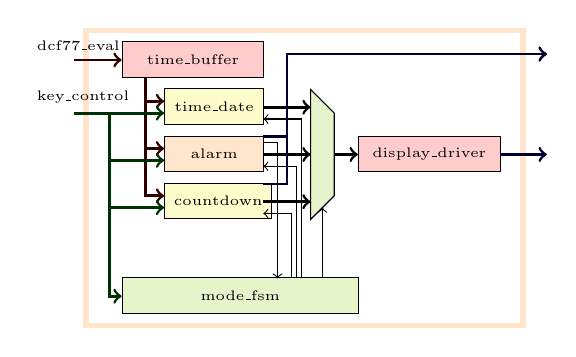
\begin{tikzpicture}[x=.6cm,y=.6cm,font=\tiny]
				% top level module
				\draw[white!80!orange,line width=2pt] (-.75,0) rectangle (8.5, -6.25);

				% individual modules
				\node[rectangle,fill=white!80!red,   draw=black,minimum height=0.45cm,minimum width=1.80cm,above right] at (0.,-1) {time\_buffer};
				\node[rectangle,fill=white!80!yellow,draw=black,minimum height=0.45cm,minimum width=1.26cm,above right] at (.9,-2) {time\_date};
				\node[rectangle,fill=white!80!orange,draw=black,minimum height=0.45cm,minimum width=1.26cm,above right] at (.9,-3) {alarm};
				\node[rectangle,fill=white!80!yellow,draw=black,minimum height=0.45cm,minimum width=1.26cm,above right] at (.9,-4) {countdown};
				\node[rectangle,fill=white!80!red,   draw=black,minimum height=0.45cm,minimum width=1.80cm,above right] at (5.,-3) {display\_driver};
				\node[rectangle,fill=yellow!50!green!20!white,draw=black,minimum height=0.45cm,minimum width=3.00cm,above right] at (0.,-6) {mode\_fsm};

				% time signals
				\draw[red!19!black,line width=1pt,->] (-1,-.625) -- (0,-.625);
				\draw[red!19!black,line width=1pt,->] (.5,-1) -- (.5,-1.5) -> (.9,-1.5);
				\draw[red!19!black,line width=1pt,->] (.5,-1) -- (.5,-2.5) -> (.9,-2.5);
				\draw[red!19!black,line width=1pt,->] (.5,-1) -- (.5,-3.5) -> (.9,-3.5);
				\node[rectangle,above right] at (-2,-.625) {dcf77\_eval};

				% key status signals
				\draw[green!19!black,line width=1pt,->] (-1,-1.75) -- (-.25,-1.75) -- (-.25,-1.75) -> (.9,-1.75);
				\draw[green!19!black,line width=1pt,->] (-1,-1.75) -- (-.25,-1.75) -- (-.25,-2.75) -> (.9,-2.75);
				\draw[green!19!black,line width=1pt,->] (-1,-1.75) -- (-.25,-1.75) -- (-.25,-3.75) -> (.9,-3.75);
				\draw[green!19!black,line width=1pt,->] (-1,-1.75) -- (-.25,-1.75) -- (-.25,-5.625) -> (0,-5.625);
				\node[rectangle,above right] at (-2,-1.75) {key\_control};

				% display data signals
				\draw[line width=1pt,->] (3,-1.625) -> (4, -1.625);
				\draw[line width=1pt,->] (3,-2.625) -> (4, -2.625);
				\draw[line width=1pt,->] (3,-3.625) -> (4, -3.625);
				\draw[line width=1pt,->] (4.5,-2.625) -> (5, -2.625);

				% status signals modules -> fsm
				% only needed for alarm since we dropped the modified signal
				% \draw[->] (3,-1.375) -- (3.4,-1.375) -> (3.4,-5.25);
				\draw[->] (3,-2.375) -- (3.3,-2.375) -> (3.3,-5.25);
				% \draw[->] (3,-3.375) -- (3.2,-3.375) -> (3.2,-5.25);

				% control signals fsm -> modules
				\draw[->] (3.8,-5.25) -- (3.8,-1.875) -> (3,-1.875);
				\draw[->] (3.7,-5.25) -- (3.7,-2.875) -> (3,-2.875);
				\draw[->] (3.6,-5.25) -- (3.6,-3.875) -> (3,-3.875);

				% mux ctl
				\draw[->] (4.25,-5.25) -> (4.25,-3.75);

				% misc outputs from modules (alarm, timer)
				\draw[blue!19!black,line width=1pt,->] (3,-2.25) -- (3.5,-2.25) -- (3.5,-.5) -> (9,-.5);
				\draw[blue!19!black,line width=1pt,->] (3,-3.25) -- (3.5,-3.25) -- (3.5,-.5) -> (9,-.5);

				% \node[rectangle,draw=black,above right] at (5,-1.75) {sw\_on<='0'};
				% \draw[blue!70!black,line width=2pt,->] (6,-1.2) -- (6,-.5) -> (9,-.5);

				% display control lines
				\draw[blue!19!black,line width=1pt,->] (8,-2.625) -> (9,-2.625);

				% mux
				\draw[fill=yellow!50!green!20!white] (4,-1.25) -- (4.5, -1.75) -- (4.5,-3.5) -- (4,-4) -- cycle;
			\end{tikzpicture}
		\end{column}
	\end{columns}
\end{frame}

\begin{frame}{Common System Integration}
	\begin{itemize}
		\item Common data format: VHDL package for all modules % already created
		\item Use git to synchronize efforts
		\item E-Mail for discussion
		\item Top level module is treated like any other module
	\end{itemize}
\end{frame}

\begin{frame}{Testing strategy}
	\begin{enumerate}
		\item person assigned to module creates individual testbench
		\item test corner cases, e.g.: \begin{itemize}
			\item correct behavior when alarm is ringing
			\item invalid DCF77 signal
			\item reset
			\item continued countdown in background
		\end{itemize}
		\item supervisor checks module and testbench after realization
		\item tests on actual hardware
	\end{enumerate}
\end{frame}

\begin{frame}{Testing strategy}
	\begin{center}
		\begin{tabular}{lll}
			\toprule
									& implement   & supervise  \\ \midrule
			time\_buffer      & Mathias     & Sophia     \\
			display\_driver   & Mathias     & Sophia     \\
			mode\_fsm         & Fabian      & Tobi       \\
			display\_mux      & Fabian      & Tobi       \\
			mode\_time\_date  & Tobi        & Mathias    \\
			mode\_alarm       & Sophia      & Fabian     \\
			mode\_countdown   & Tobi        & Mathias    \\
			uhrenbaustein     & Sophia      & Fabian     \\ \bottomrule
		\end{tabular}
	\end{center}
\end{frame}

\begin{frame}{Display Timing}
	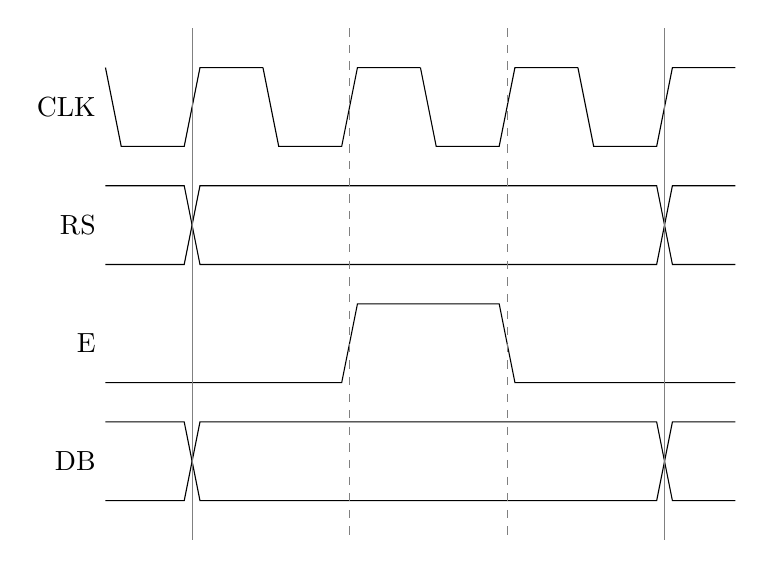
\begin{tikzpicture}
		\foreach \x in {0,2,4,6} \draw (\x-0.1,1) -- (\x+0.1,0) -- (\x+0.9,0) -- (\x+1.1,1) -- (\x+1.9,1);
		\draw (-0.1,-1.5) -- (0.9,-1.5) -- (1.1,-0.5) -- (6.9,-0.5) -- (7.1,-1.5) -- (7.9,-1.5);
		\draw (-0.1,-0.5) -- (0.9,-0.5) -- (1.1,-1.5) -- (6.9,-1.5) -- (7.1,-0.5) -- (7.9,-0.5);

		\draw (-0.1,-3.0) -- (2.9,-3.0) -- (3.1,-2.0) -- (4.9,-2.0) -- (5.1,-3.0) -- (7.9,-3.0);

		\draw (-0.1,-4.5) -- (0.9,-4.5) -- (1.1,-3.5) -- (6.9,-3.5) -- (7.1,-4.5) -- (7.9,-4.5);
		\draw (-0.1,-3.5) -- (0.9,-3.5) -- (1.1,-4.5) -- (6.9,-4.5) -- (7.1,-3.5) -- (7.9,-3.5);

		\node[left] at (-.1, 0.5) {CLK};
		\node[left] at (-.1,-1.0) {RS};
		\node[left] at (-.1,-2.5) {E};
		\node[left] at (-.1,-4.0) {DB};

		\draw[gray] (1,1.5) -- (1,-5);
		\draw[gray,dashed] (3,1.5) -- (3,-5);
		\draw[gray,dashed] (5,1.5) -- (5,-5);
		\draw[gray] (7,1.5) -- (7,-5);
	\end{tikzpicture}
\end{frame}

\begin{frame}{Display Driver Overview}
	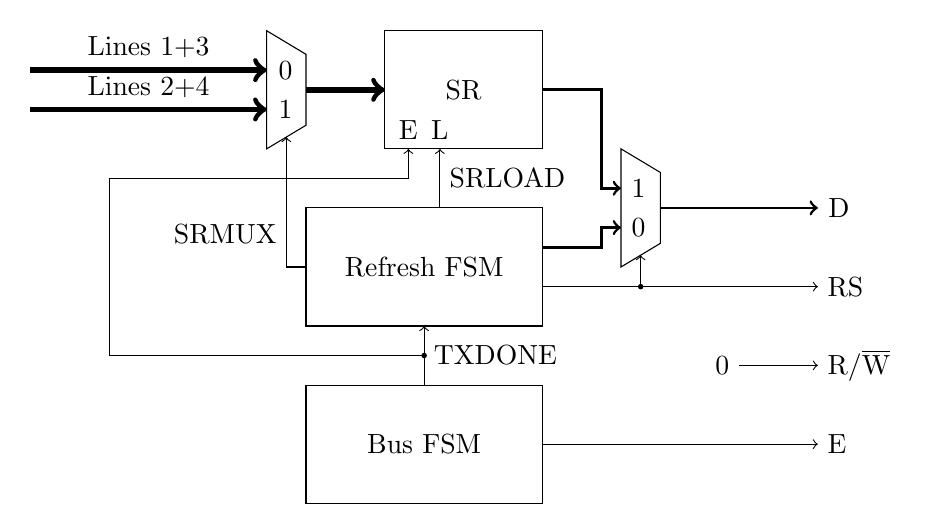
\begin{tikzpicture}
		\draw[line width=2pt,->] (0,0) -> (3, 0) node[midway,above] {Lines 1+3} node[right] {0};
		\draw[line width=2pt,->] (0,-.5) -> (3, -.5) node[midway,above] {Lines 2+4} node[right] {1};
		\draw[line width=2pt,->] (3.5,-.25) -> (4.5,-.25);
		\draw[line width=1pt,->] (6.5,-.25) -- (7.25,-.25) -- (7.25,-1.5) -> (7.5,-1.5) node[right] {1};
		\draw[line width=1pt,->] (6.5,-2.25) -- (7.25,-2.25) -- (7.25,-2) -> (7.5,-2) node[right] {0};
		\draw[line width=1pt,->] (8,-1.75) -> (10,-1.75) node[right] {D};

		\draw (3,.5) -- (3.5,.2) -- (3.5,-.7) -- (3,-1) -- cycle;

		\node at (5.5, -.25) {SR};
		\draw (4.5,.5) rectangle (6.5,-1);

		\node at(5,-2.5) {Refresh FSM};
		\draw (3.5,-1.75) rectangle (6.5,-3.25);

		\node at(5,-4.75) {Bus FSM};
		\draw (3.5,-4) rectangle (6.5,-5.5);

		\draw[->] (5,-4) -> (5,-3.25) node[right,midway] {TXDONE};
		\draw[->] (5,-3.625) -- (1,-3.625) -- (1,-1.375) -- (4.8, -1.375) -> (4.8, -1) node[above] { E };
		\fill (5,-3.625) circle (1pt);

		\draw[->] (3.5,-2.5) -- (3.25,-2.5) -> (3.25,-.85) node[left,near start] {SRMUX};

		\draw[->] (5.2,-1.75) -> (5.2,-1) node[above] {L} node[midway,right] {SRLOAD};

		\draw (7.5,-1.0) -- (8,-1.3) -- (8,-2.2) -- (7.5,-2.5) -- cycle;

		\draw[->] (6.5,-2.75) -> (10,-2.75) node[right] {RS};
		\draw[->] (7.75,-2.75) -> (7.75,-2.35);
		\fill (7.75,-2.75) circle (1pt);
		\draw[->] (6.5,-4.75) -> (10,-4.75) node[right] {E};
		\draw[->] (9,-3.75) node[left] {0} -> (10,-3.75) node[right] {R/$\overline{\text{W}}$};
	\end{tikzpicture}
\end{frame}

\begin{frame}{Display Driver Bus FSM}
	\begin{center}
		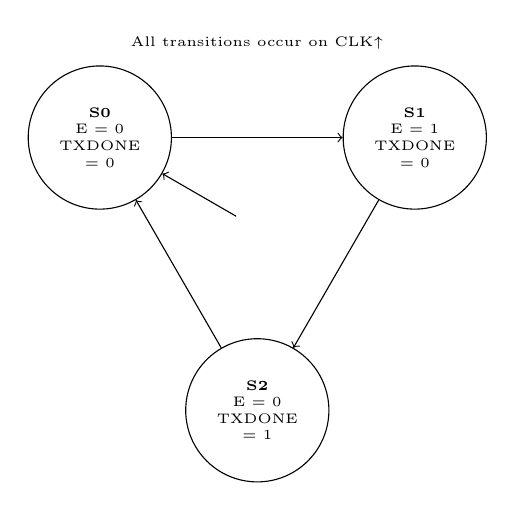
\begin{tikzpicture}[every state/.style={text width=1.3cm,align=center,node distance=.5cm},font=\tiny,auto]
			\node at (2,1.2) {All transitions occur on CLK$\uparrow$};
			\node[state] (S0) at (0.0,0) { \textbf{S0} \\ E = 0 \\ TXDONE = 0 };
			\node[state] (S1) at (4.0,0) { \textbf{S1} \\ E = 1 \\ TXDONE = 0 };
			\node[state] (S2) at (-60:4) { \textbf{S2} \\ E = 0 \\ TXDONE = 1 };

			\path[->] (S0) edge (S1)
						 (S1) edge (S2)
						 (S2) edge (S0)
						 (S0) ++ (-30:2) edge (S0);
		\end{tikzpicture}
	\end{center}
\end{frame}

\begin{frame}{Display Driver Refresh FSM}
	\begin{center}
		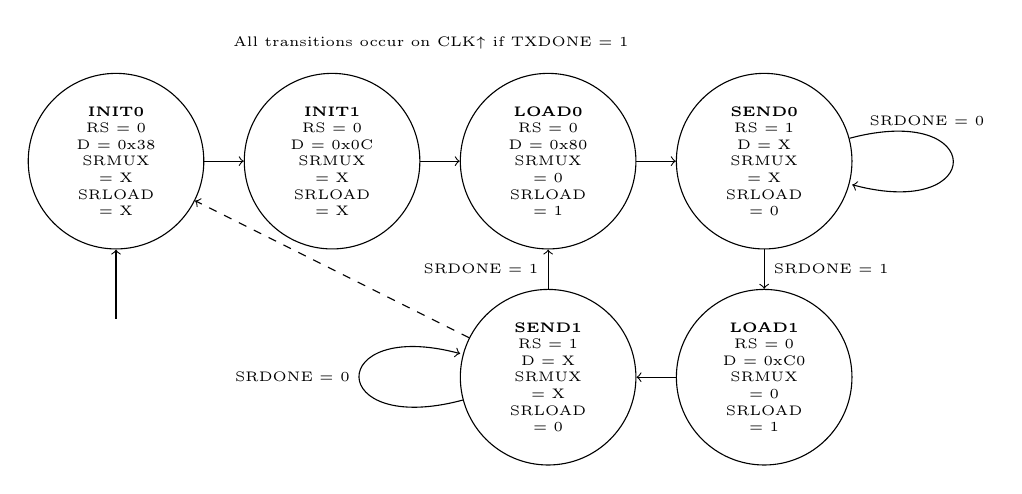
\begin{tikzpicture}[every state/.style={text width=1.3cm,align=center,node distance=.5cm},font=\tiny,auto]
			\node at (4,1.5) {All transitions occur on CLK$\uparrow$ if TXDONE = 1};
			\node[state]                       (FunctionSet)  { \textbf{INIT0} \\ RS = 0 \\ D = 0x38 \\ SRMUX = X \\ SRLOAD = X };
			\node[state,right=of FunctionSet]  (DisplayOnOff) { \textbf{INIT1} \\ RS = 0 \\ D = 0x0C \\ SRMUX = X \\ SRLOAD = X };
			\node[state,right=of DisplayOnOff] (SetAddrUpper) { \textbf{LOAD0} \\ RS = 0 \\ D = 0x80 \\ SRMUX = 0 \\ SRLOAD = 1 };
			\node[state,right=of SetAddrUpper] (WriteUpper)   { \textbf{SEND0} \\ RS = 1 \\ D = X    \\ SRMUX = X \\ SRLOAD = 0 };
			\node[state,below=of WriteUpper]   (SetAddrLower) { \textbf{LOAD1} \\ RS = 0 \\ D = 0xC0 \\ SRMUX = 0 \\ SRLOAD = 1 };
			\node[state,left =of SetAddrLower] (WriteLower)   { \textbf{SEND1} \\ RS = 1 \\ D = X    \\ SRMUX = X \\ SRLOAD = 0 };

			\path[->] (FunctionSet) ++(0,-2) edge (FunctionSet)
						 (FunctionSet)  edge                                  (DisplayOnOff)
						 (DisplayOnOff) edge                                  (SetAddrUpper)
						 (SetAddrUpper) edge                                  (WriteUpper)
						 (WriteUpper)   edge             node {SRDONE = 1}    (SetAddrLower)
											 edge[loop right,near start,above] node {SRDONE = 0} ()
						 (SetAddrLower) edge                                  (WriteLower)
						 (WriteLower)   edge             node {SRDONE = 1}    (SetAddrUpper)
											 edge[loop left]  node {SRDONE = 0}    ();
			\path[->,dashed]
						 (WriteLower)   edge                                  (FunctionSet);
		\end{tikzpicture}
	\end{center}
\end{frame}

\begin{frame}{Clock Buffer Circuit}
	\begin{center}
		\begin{tikzpicture}
			\tikzset{dcf update/.style={}}
			\tikzset{dcf update fill/.style={}}
			\tikzset{counter update/.style={}}
			\tikzset{counter update fill/.style={}}
			\only<2> {
				\tikzset{dcf update/.style={color=red}}
				\tikzset{dcf update fill/.style={fill=red}}
			}
			\only<3> {
				\tikzset{counter update/.style={color=red}}
				\tikzset{counter update fill/.style={fill=red}}
			}

			\node[rectangle,draw=black,minimum height=0.75cm,minimum width=4cm,above right] at (0,-1) {+ 1 min, valid <= 0};
			\node[rectangle,draw=black,minimum height=2.75cm,minimum width=1cm,above right] at (2,-4) {};
			\node[rectangle,draw=black,minimum height=0.75cm,minimum width=1cm,above right] at (0,-3.5) {$\geq 1$};
			\node[rectangle,draw=black,minimum height=0.75cm,minimum width=1cm,above right] at (-.25,-5.5) {$\geq 1$};
			\node[rectangle,draw=black,minimum height=0.75cm,minimum width=2.25cm,above right] at (1,-5.5) {counter};
			\node[rectangle,draw=black,minimum height=0.75cm,minimum width=2.75cm,above right] at (3.5,-5.5) {= 59999};

			\draw (.75,-1.25) -- (1.25,-1.50) -- (1.25,-2.25) -- (.75,-2.50) -- cycle;

			% time signals
			\draw[red!50!black,line width=2pt,->,counter update] (0,-0.625) -- (-.25,-0.625) -- (-.25,-1.666667) -> (.75,-1.666667) node[right,black,counter update] {0};
			\draw[red!50!black,line width=2pt,->,dcf update] (-1,-2.083333) node[left,black] {DCF77\_dec} -> (.75,-2.083333) node[right,black,dcf update] {1};
			\draw[red!50!black,line width=2pt,->, dcf update,counter update] (1.25,-1.875) -> (2,-1.875) node[right,black,dcf update,counter update] {D};
			\draw[red!50!black,line width=2pt,->] (4.25,-1.875) -- (7,-1.875);
			\draw[red!50!black,line width=2pt,->,counter update] (3,-1.875) node[left,black] {Q} -- (4.25,-1.875) -- (4.25,-.625) -> (4,-.625);

			% OR gate outputs
			\draw[->,dcf update,counter update] (1,-3.125) -> (2,-3.125) node[right] {E};
			\draw[->,dcf update,counter update] (1.5,-3.125) -- (1.5,-3.75) -- (-.5,-3.75) -- (-.5,-5) -> (-.25,-5);
			\fill[dcf update fill,counter update fill] (1.5,-3.125) circle (1pt);
			\draw[->,dcf update,counter update] (.75,-5.125) -> (1,-5.125) node[right] {R};
			\draw[->] (-.75,-4.25) -- (-.75,-5.25) -> (-.25,-5.25);

			% OR gate / MUX inputs
			\fill[dcf update fill] (-.25,-2.083333) circle (1pt);
			\draw[->,dcf update] (-.25,-2.083333) -- (-.25,-3) -> (0,-3);
			\draw[->,dcf update] (-.25,-2.625) -- (1,-2.625) -> (1,-2.375);
			\fill[dcf update fill] (-.25,-2.625) circle (1pt);
			\draw[->,counter update] (6.25,-5.125) -- (6.5,-5.125) -- (6.5,-4.5) -- (-.25,-4.5) -- (-.25,-3.25) -- (0,-3.25);

			% counter value
			\draw[->,line width=2pt] (3.25,-5.125) -> (3.5,-5.125);

			% clock and reset lines
			\draw[white!50!black,line width=2pt] (-1,-4.25) node[left,black] {clk, reset} -- (3.25,-4.25);
			\draw[->] (2.333333,-4.25) -- (2.333333,-4) node[above] {R};
			\draw[->] (2.666667,-4.25) -- (2.666667,-4);
			\draw (2.666667,-4) +(0.173205,0) -- +(0,.2) -- +(-0.173205,0);
			\draw[->] (3,-4.25) ->  (3,-4.75);
			\draw (3,-4.75) +(0.173205,0) -- +(0,-.2) -- +(-0.173205,0);
			\fill (2.333333,-4.25) circle (1pt);
			\fill (2.666667,-4.25) circle (1pt);
			\fill (3,-4.25) circle (1pt);
			\fill (-.75,-4.25) circle (1pt);

		\end{tikzpicture}
	\end{center}
\end{frame}

\end{document}
